\documentclass[landscape,xcolor={table}]{beamer}

\usepackage{amsmath}
\usepackage{graphicx}
\usepackage[english]{babel}
\usetheme{Antibes}
\usepackage{tikz}



\usetheme{default}
\usecolortheme{albatross}
\usefonttheme[onlymath]{serif}
\setbeamertemplate{caption}[numbered]
\graphicspath{ {images/} }

\pgfdeclareimage[width=\paperwidth]{mybackground}{images/blue_sun.png}

\setbeamertemplate{title page}{

        \begin{picture}(0,0)

            \put(-30,-163){%
                \pgfuseimage{mybackground}
            }

            \put(0,-110.7){%
                \begin{minipage}[b][45mm][t]{226mm}
                    \usebeamerfont{title}{\inserttitle\par}
                \end{minipage}
            }

            \end{picture}

    }

\title[...]{Hardware and Software Development for \\ MOSES II Flight Operations}
\author[Smart, Mashburn]{Roy Smart \and Jackson Remington}
\institute{Montana State University}
\date{May 1st, 2015}


	
\begin{document}

	\begin{frame}[plain]
	        \titlepage
	\end{frame}
	
	\begin{frame}
		
		\frametitle{MOSES Scientific Goals}

	\end{frame}
	
	\begin{frame}
		
		\frametitle{First Launch}

	\end{frame}

	\begin{frame}
		
		\frametitle{System Requirements}

	\end{frame}
	
	\begin{frame}
		
		\frametitle{Hardware Overview}

	\end{frame}
	
	\begin{frame}
		
		\frametitle{Flight Software}

	\end{frame}
	
	\begin{frame}
		
		\frametitle{Ground Station Software}
		
		\noindent
		\begin{minipage}[t]{.5\textwidth}
		  
		  \begin{itemize}
		  	\item{Server module}
		  	\item{Client module}
		  	\item{Grounded communication}
		  	\begin{itemize}
		  		\item{Serial console}
		  		\item{Ethernet}
		  	\end{itemize}
		  	\item{In-flight communication}
			\begin{itemize}
		  		\item{Housekeeping Link Protocol (HLP)}
		  		\item{Timers}
		  		\item{High-speed telemetry}
		  	\end{itemize}
		  \end{itemize}
		\end{minipage}
		
		\begin{minipage}[t]{.44\textwidth}
		  
		  \begin{figure}
		  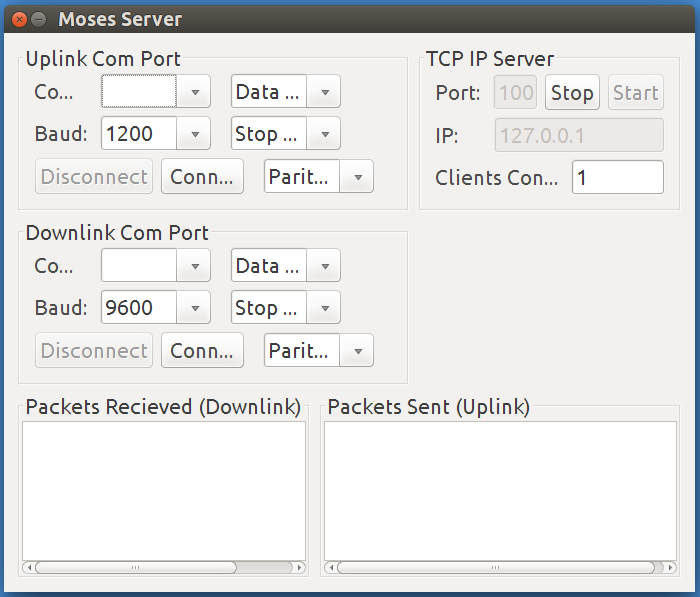
\includegraphics[width=\textwidth]{server_scr}
		  \end{figure}
		  \begin{figure}
 		  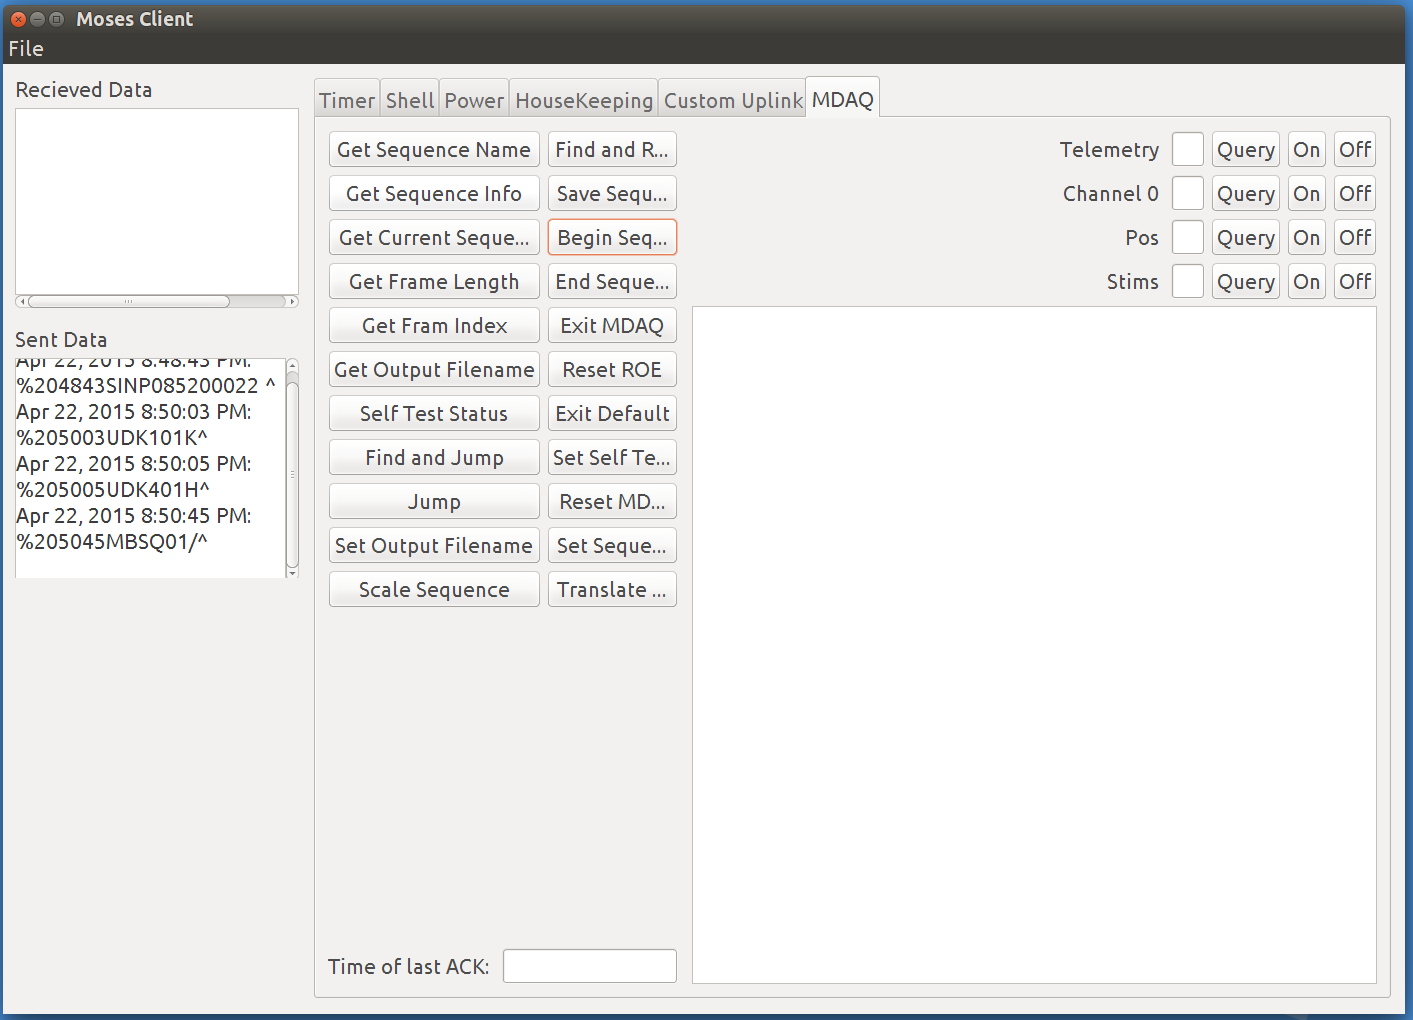
\includegraphics[width=\textwidth]{client_scr}
 		  \end{figure}
		
		\end{minipage}
		
		

	\end{frame}
	
	\begin{frame}
		
		\frametitle{Capturing Data}

	\end{frame}
	
	\begin{frame}
		
		\frametitle{Data Retrieval}

	\end{frame}
	
	\begin{frame}
		
		\frametitle{Next Launch}

	\end{frame}
	
\end{document}








